% !TeX spellcheck = en_US 
\section{Introduction}\label{interlocking:sec:intro}
Multi-material \revise{FDM 3D printers}{extrusion 3D printers} unlock a plethora of applications through combining the unique material properties of various materials.
However, depending on the combination of materials the adhesion between the materials can be excessively weak.
While only a small number of all possible 3D printing material combinations may exhibit any incompatibility issues,
it is often precisely those incompatible combinations where the different chemical make-up produces interesting applications.
For example, polypropylene (PP) is semi-flexible and fatigue-resistant, but has a very weak chemical bond to typical rigid filaments such as polylactic acid (PLA).
PP is often used for living hinges, which consist of a single part rather than moving components.
Combining these materials unlocks compliant mechanism applications such as visualized in \cref{interlocking:fig:applications}.
In such cases it is necessary to rely on mechanical interlocking to prevent the materials from breaking apart from each other.


\begin{figure}
	\centering
	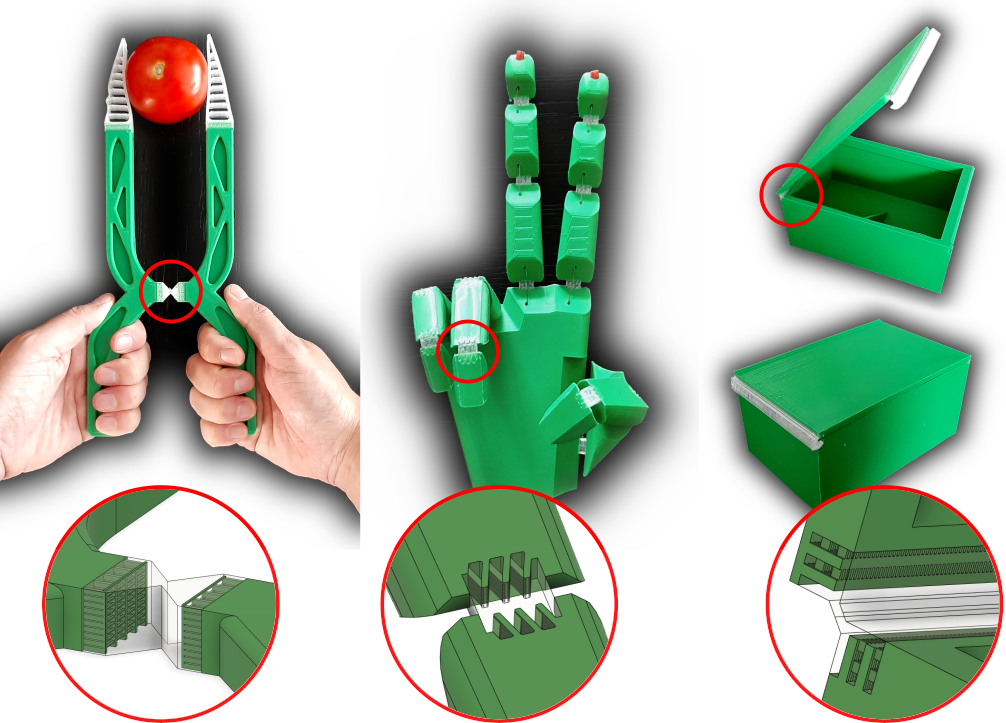
\includegraphics[width=\columnwidth]{sources-applications-applications.png}
	\caption{Applications of dual material products using the ITI\revise{M}{L} lattice for interlocking Ultimaker transparent PP and Ultimaker green tough PLA material.
	A gripper making use of the straight ITI\revise{M}{L} variant.
	A prosthetic hand using the diagonal ITI\revise{M}{L} variant.
	A storage box utilizing the straight ITI\revise{M}{L} variant.
	}
	\label{interlocking:fig:applications}
\end{figure}





\begin{figure}
	\centering
	\setlength{\figheight}{.45\columnwidth}\centering
	\begin{subfigure}[B]{.25\columnwidth}
		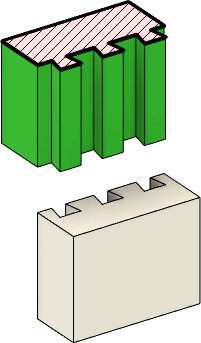
\includegraphics[height=\figheight]{sources-method-basic_2d_interlock.jpg}
		\caption{A 2D dovetail interlock}
		\label{interlocking:fig:basic_2d_interlock}
	\end{subfigure}
	\begin{subfigure}[B]{.36\columnwidth}\centering
		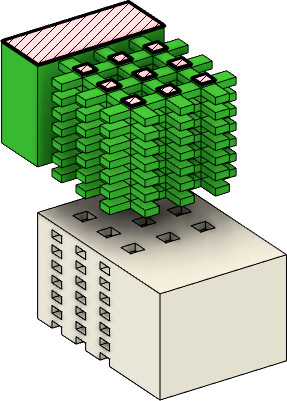
\includegraphics[height=\figheight]{sources-method-discontinuous_lattice.jpg}
		\caption{Cubic lattice with disconnected islands}
		\label{interlocking:fig:discontinuous_lattice}
	\end{subfigure}
	\begin{subfigure}[B]{.36\columnwidth}\centering
		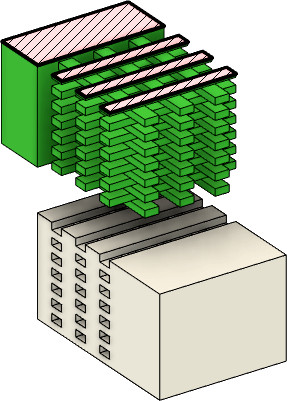
\includegraphics[height=\figheight]{sources-method-basic_lattice.jpg}
		\caption{The ITI\revise{M}{L} lattice with long continuous paths}
		\label{interlocking:fig:basic_structure_single_mat}
	\end{subfigure}
	\caption{Interlocking principles; exploded view with a section cut at the top layer. The dovetail can be disassembled by translation; the cubic lattice causes highly discontinuous extrusion on some layers; the proposed ITI\revise{M}{L} lattice solves these problems.}
	\label{interlocking:fig:basic_structure}
\end{figure}





Dovetail interlocking is a common strategy to affix two bodies together;
one example can be found in jigsaw puzzles.
The pieces interlock and stay connected because of the material stiffness.
However, the interlock can be broken in plane by deformation of the pieces,
and out of plane the pieces can be disassembled by translation alone.
See \cref{interlocking:fig:basic_2d_interlock}.
Moreover, because the dovetails widen toward their tip, they cannot easily be printed with continuous extrusion toolpaths.

In order to overcome these limitations, we propose \emph{topological interlocking}\revise{.
For topologically interlocking structures }
{, which is a type of interlocking where the interlock is preserved under continuous deformations such as stretching, twisting or bending of any magnitude 
-- that is: the bodies can only be unlocked by discontinuous deformations such as fracture.
In order to achieve topological interlocking both materials have a high genus topology:}
the holes or tunnels in one material are filled with the other material and vice versa,
\revise{thereby creating a structure where the two materials are linked together}{}similar to \revise{}{how the rings of }chain mail\revise{}{ are linked together}.\revise{
Chain mail cannot be disassembled by continuous deformations such as stretching, twisting or bending,
because the presence of holes or tunnels is preserved under any such deformations.}{}
A topological interlock remains effective under any deformation of the base materials and can only be broken by failure in either material.
This interlocking principle is robust especially when flexible and deformable materials are concerned.

\revise{}{The concept of topological interlocking should not be confused with the homonymous term which refers to interlocking assemblies, where blocks ``of special shape are arranged in such a way that the whole structure can be held together by a global peripheral constraint [such as compression], while locally the elements are kept in place by kinematic constrains imposed through the shape and mutual arrangement of the elements.''\cite{Estrin2011} % first introduction of the term: dyskin2001toughening
In contrast, this paper pertains to bodies of different materials which interlock by topological constraints and optimizes for a globally applied tension.}

%We propose a topologically interlocking structure where all voids in the one material are filled with the other material and vice versa.
However, most topologically interlocking geometries would introduce discontinuities in the extrusion process when sliced into layers for 3D printing, as each slice would contain disconnected islands.
See \cref{interlocking:fig:discontinuous_lattice}.
Such discontinuities can easily lead to defects, which influence the dimensional accuracy and the mechanical properties of the resulting part.
% Moreover, depositing small disconnected islands of one material on top of a chemically incompatible material cannot reliably be performed because of the weak bonding.
We therefore have to generate interlocking geometry for which the layers consist of long continuously connected areas for both materials.

It seems impossible to generate topologically interlocking geometry with holes or tunnels while enforcing continuous extrusion for both materials;
if the one material leaves a hole in a layer then filling that hole with the other material will cause it to be disconnected from the other regions of the second material.
The ITI\revise{M}{L} lattice consists of long horizontal beams which ensure continuous extrusion, which alternate in orientation along the Z axis in order to connect all beams together, thereby creating linked hoops which constitute the topological interlock.
Where the beams of the two orientations meet they form long vertical pillars. %, which constitute vertical tunnels in the other material.
However, the small island cross-sections of these pillars are all located in between consecutive layers, so that they never result in disconnected islands.
See \cref{interlocking:fig:basic_structure_single_mat}.


Our contributions are as follows:
\begin{itemize}
	\item An interlaced topologically interlocking \revise{microstructure}{lattice} (ITI\revise{M}{L}) which satisfies the extrusion continuity constraint.
	\item Two variants of the ITI\revise{M}{L} lattice optimized for tensile forces: straight and diagonal.
	\item A theoretical upper bound to the tensile strength of any interlocking structure.
	\item Analytical models for estimating tensile properties and for optimizing the design parameters of the interlocking structures.
	\item Numerical and experimental validation.
\end{itemize}






